\documentclass[tikz,border=1pt]{standalone}
\usepackage{mathptmx}  % Times, as in the paper preamble
\usetikzlibrary{patterns,arrows.meta,shapes.geometric}
\begin{document}
\footnotesize
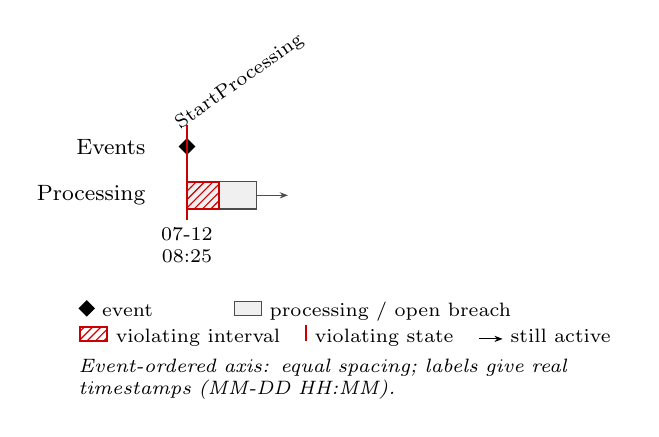
\begin{tikzpicture}[x=1.35cm,y=-0.62cm,
  lane/.style={anchor=east,font=\footnotesize},
  basis/.style={fill=black!18,draw=black!70},
  proc/.style={fill=black!6,draw=black!70},
  breach/.style={fill=black!6,draw=black!70},
  unlawful/.style={pattern=north east lines,pattern color=red!80!black,draw=red!80!black,thick},
  overdue/.style={pattern=north east lines,pattern color=red!80!black,draw=red!80!black,thick},
  ev/.style={fill=black,draw=black,diamond,inner sep=1.4pt},
  tick/.style={font=\scriptsize,align=center,anchor=north,inner sep=1pt}]

\draw[black!15] (0,-0.45) -- (0,1.50);
\node[tick] at (0,1.60) {07-12\\08:25};
\node[lane] at (-0.3,0) {Events};
\node[lane] at (-0.3,1) {Processing};
\draw[proc] (0.00,0.72) rectangle (0.65,1.28);
\draw[-{Stealth[length=3pt]},black!70] (0.65,1) -- ++(0.3,0);
\draw[unlawful] (0.00,0.72) rectangle (0.30,1.28);
\node[ev] at (0,0) {};
\node[font=\scriptsize,anchor=south west,rotate=35,inner sep=1pt] at (-0.05,-0.2) {StartProcessing};
\draw[red!80!black,thick] (0,-0.45) -- (0,1.50);
\node[anchor=north west,font=\scriptsize,text width=6.90cm,xshift=-1.5cm] at (0,2.95) {\mbox{\tikz[x=1cm,y=1cm]\node[ev]{}; event}\hspace{0.8em plus 1em} \mbox{\tikz[x=1cm,y=1cm]\draw[proc](0,0)rectangle(.35,.18); processing / open breach}\hspace{0.8em plus 1em} \mbox{\tikz[x=1cm,y=1cm]\draw[unlawful](0,0)rectangle(.35,.18); violating interval}\hspace{0.8em plus 1em} \mbox{\tikz[x=1cm,y=1cm]\draw[red!80!black,thick](0,0)--(0,.2); violating state}\hspace{0.8em plus 1em} \mbox{\tikz[x=1cm,y=1cm]\draw[-{Stealth[length=3pt]}](0,.1)--(.3,.1); still active}\par\smallskip\textit{Event-ordered axis: equal spacing; labels give real timestamps (MM-DD HH:MM).}};
\end{tikzpicture}
\end{document}
